\section{Specifica dei test}
Il \textit{team\ped{G}} \gruppo, al fine di implementare del software che sia di qualità, ha strutturato dei test atti a verificare che il software prodotto rispecchi le funzionalità a fronte di risultati attesi.
Questi test sono il frutto dell'applicazione delle tecniche di verifica dinamica che sono state introdotte nel documento \NdP.
Tutte le attività di testing prodotte devono poter essere ripetibili e devono essere deterministiche, al fine di poter fornire delle informazioni utili a intraprendere azioni di correzione, nel caso in cui i risultati ottenuti siano diversi da quelli attesi.
Per avere un tracciamento dei test prodotti e dei risultati ottenuti si è scelto di classificare il tutto producendo dei log che siano di facile consultazione e che possano fornire una precisa indicazione di quelli che sono stati gli output di queste attività di verifica, eventuali errori o eventuali risultati che siano non coerenti con quanto in precedenza fissato.
\subsection{Tipi di test}
Sono stati individuati quattro livelli di testing e sono rispettivamente:
\begin{itemize}
\item \textbf{Test di unità [TU]:} con questa tipologia di test si cerca di verificare la più piccola parte di lavoro prodotta da un programmatore. Questo si traduce tendenzialmente a verificare i metodi e le funzioni scritte;
\item \textbf{Test di integrazione [TI]:} con questa tipologia di test si cerca di verificare le componenti di sistema. Più precisamente, l'obiettivo è quello di testare il funzionamento dei vari package prodotti, sia singolarmente che nel loro insieme;
\item \textbf{Test di sistema [TS]:} con questa tipologia di test si cerca di verificare che il comportamento e il funzionamento dell'architettura siano corretti;
\item \textbf{Test di validazione [TV]:} con questa tipologia di test si vuole verificare che il lavoro prodotto soddisfi quanto richiesto dal proponente.
\end{itemize}

% INSERIMENTO DEI TEST
\subsubsection{Test di Validazione}
I test di validazione hanno lo scopo di accertare che tutte le funzionalità richieste dal proponente siano state soddisfatte. Per questo motivo, attraverso delle macro azioni, si andrà a simulare il comportamento generale dell'applicativo e dell'utente che interagisce con esso.
I test di validazione saranno organizzati nel modo seguente:
\begin{center}
\textbf{TV}[\textit{TipoRequisito}][\textit{ImportanzaRequisito}][\textit{IdRequisito}]
\end{center}
dove:
\begin{itemize}
\item
\textbf{TipoRequisito} può assumere valori tra:
	\begin{itemize}
	\item
	\textit{F} per i requisiti funzionali;
	\item
	\textit{Q} per i requisiti di qualità;
	\item
	\textit{V} per i requisiti di vincolo;
	\item
	\textit{P} per i requisiti prestazionali.
	\end{itemize}
\item 
\textbf{ImportanzaRequisito} può assumere valori tra:
	\begin{itemize}
	\item
	\textit{D} per i requisiti desiderabili;
	\item
	\textit{O} per i requisiti di obbligatori;
	\item
	\textit{F} per i requisiti di facoltativi.
	\end{itemize}
\item
\textbf{IdRequisito} assume un valore gerarchico che identifica il singolo requisito.
\end{itemize}

% TABELLA
\normalsize
\begin{longtable}[ht]{|c|>{}m{8cm}|c|}
\hline 
\textbf{Id Test} & \textbf{Descrizione} & \textbf{Stato}\\
\hline
\endhead
\hypertarget{TVFO1}{TVFO1} & L’utente intende registrarsi al sistema. All’utente è richiesto di:
\begin{itemize}
\item
Trovarsi nella sezione apposita;
\item
Compilare il form di registrazione;
\item
Premere il pulsante di conferma.
\item
Verificare attraverso l’autenticazione che la registrazione sia effettivamente avvenuta.
\end{itemize}
 & \textit{Non Implementato}\\ \hline
\hypertarget{TVFO2}{TVFO2} & L’utente intende autenticarsi al sistema. All’utente è richiesto di:
\begin{itemize}
\item
Trovarsi nella sezione apposita;
\item
Inserire le credenziali nell’apposito form;
\item
Premere il pulsante di autenticazione;
\item
Verificare che l’autenticazione sia effettivamente avvenuta.
\end{itemize}
 & \textit{Non Implementato}\\ \hline
\hypertarget{TVFO3}{TVFO3} & L’utente intende disconnettersi dal sistema. All’utente è richiesto di:
\begin{itemize}
\item
Essere Autenticato;
\item
Trovarsi nella sezione apposita;
\item
Premere il pulsante di logout;
\item
Verificare che la disconnessione sia effettivamente avvenuta. 
\end{itemize}
& \textit{Non Implementato}\\ \hline
\hypertarget{TVFD4}{TVFD4} & L’utente autenticato  intende gestire i propri dati. All’utente è richiesto di:
\begin{itemize}
\item
Essere autenticato;
\item
Trovarsi nella sezione apposita;
\item
Modificare i campi dati consentiti;
\item
Premere il tasto conferma modifica;
\item
Visualizzare il profilo dell'utente modificato.
\end{itemize}
 & \textit{Non Implementato}\\ \hline
\hypertarget{TVFD4.3}{TVFD4.3} & L’utente autenticato  intende impostare la propria foto profilo . All’utente è richiesto di:
\begin{itemize}
\item
Essere autenticato;
\item
Trovarsi nella sezione apposita;
\item
Impostare la foto da inserire;
\item
Visualizzare il profilo dell’utente modificato.
\end{itemize}
 & \textit{Non Implementato}\\ \hline
\hypertarget{TVFD4.8}{TVFD4.8} & L’utente autenticato  intende modificare la tipologia di utenza. All’utente è richiesto di:
\begin{itemize}
\item Essere autenticato;
\item Trovarsi nella sezione apposita;
\item Cambiare la tipologia di utenza;
\item Verificare la modifica effettuata. 
\end{itemize}& \textit{Non Implementato}\\ \hline
\hypertarget{TVFD4.9}{TVFD4.9} & L’utente autenticato  intende eliminare il proprio account. All’utente è richiesto di:
\begin{itemize}
\item Essere autenticato;
\item Trovarsi nella sezione apposita;
\item Premere il tasto di elimanazione;
\item Verificare la disconnessione della sessione sia avvenuta;
\item Verificare che l’autenticazione con le credenziali dell’utente eliminato non avvenga.
\end{itemize} & \textit{Non Implementato}\\ \hline
\hypertarget{TVFD5}{TVFD5} & L’utente autenticato  intende ricercare un questionario per iscriversi. All'utente è richiesto di:
\begin{itemize}
\item Essere autenticato;
\item Trovarsi nella sezione apposita;
\item Ricercare un questionario;
\item Iscrizione ad un questionario trovato mediante l’apposito tasto;
\item Verificare l'operazione appena effettuata.
\end{itemize}
 & \textit{Non Implementato}\\ \hline
\hypertarget{TVFO6}{TVFO6} & L’utente autenticato  intende compilare un questionario a cui si è  iscritto. All’utente è richiesto di:
\begin{itemize}
\item Essere autenticato;
\item Trovarsi nella sezione apposita;
\item Selezionare il questionario da compilare;
\item Rispondere alle domande previste;
\item Confermare le risposte date al questionario;
\item Verificare il risultato del questionario.
\end{itemize}
 & \textit{Non Implementato}\\ \hline
\hypertarget{TVFD7.1}{TVFD7.1} & L’utente autenticato intende creare una nuova
domanda tramite procedura guidata. All’utente è richiesto di:
\begin{itemize}
\item Essere autenticato;
\item Trovarsi nella sezione apposita;
\item Premere il pulsante Crea nuova domanda;
\item Inserire i dati necessari alla creazione di una nuova domanda;
\item Premere il pulsante di conferma creazione
nuova domanda;
\item Verificare che sia stato creata la nuova domanda.
\end{itemize}

 & \textit{Non Implementato}\\ \hline
\hypertarget{TVFD7.2}{TVFD7.2} & L’utente autenticato intende modificare una
domanda esistente tramite procedura guidata. All’utente è richiesto di:
\begin{itemize}
\item Essere autenticato;
\item Trovarsi nella sezione apposita;
\item Premere il pulsante  modifica domanda;
\item Modificare i dati della domanda selezionata;
\item Premere il pulsante di conferma modifica;
\item Verificare che sia stata modificata la domanda.
\end{itemize}
 & \textit{Non Implementato}\\ \hline
\hypertarget{TVFO7.3}{TVFO7.3} & L’utente autenticato intende creare una nuova
domanda tramite QML. All’utente è richiesto di:
\begin{itemize}
\item Essere autenticato;
\item Trovarsi nella sezione apposita;
\item Premere il pulsante Crea nuova domanda;
\item Inserire i dati necessari alla creazione di una nuova domanda;
\item Premere il pulsante di conferma creazione
nuova domanda;
\item Verificare che sia stato creata la nuova domanda.
\end{itemize}
 & \textit{Non Implementato}\\ \hline
\hypertarget{TVFD7.4}{TVFD7.4} & L’utente autenticato intende modificare una
domanda esistente tramite QML. All’utente è richiesto di:
\begin{itemize}
\item Essere autenticato;
\item Trovarsi nella sezione apposita;
\item Premere il pulsante  modifica domanda;
\item Modificare i dati della domanda selezionata;
\item Premere il pulsante di conferma modifica;
\item Verificare che sia stata modifcata la domanda.
\end{itemize}
 & \textit{Non Implementato}\\ \hline
\hypertarget{TVFD8.1}{TVFD8.1} & L’utente autenticato intende visualizzare i questionari creati. All’utente è richiesto di:
\begin{itemize}
\item
Essere autenticato;
\item
Trovarsi nella sezione apposita;
\item
Verificare che vengano visualizzati tutti i questionari creati
\end{itemize}
 & \textit{Non Implementato}\\ \hline
\hypertarget{TVFD8.2}{TVFD8.2} & 
L’utente autenticato pro  intende modificare un questionario esistente. All’utente è richiesto di:
\begin{itemize}
\item Essere autenticato pro;
\item Trovarsi nella sezione apposita;
\item Selezionare il questionario da modificare tra quelli creati;
\item Dalla sezione di modifica effettuare tutte le modifiche consentite dal sistema 
\item Premere il pulsante di conferma modifiche;
\item Verificare che sia stato modificato il questionario correttamente.
\end{itemize}
 & \textit{Non Implementato}\\ \hline
\hypertarget{TVFD8.3}{TVFD8.3} & L’utente autenticato pro  intende eliminare un questionario esistente. All’utente è richiesto di:
\begin{itemize}
\item Essere autenticato pro;
\item Trovarsi nella sezione apposita;
\item Selezionare un questionario esistente da eliminare;
\item Premere il tasto di conferma eliminazione;
\item Verificare l’operazione appena effettuata. 
\end{itemize}
& \textit{Non Implementato}\\ \hline
\hypertarget{TVFD8.4}{TVFD8.4} & L’utente autenticato pro  intende controllare i risultati degli esaminandi di un suo questionario. All’utente è richiesto di:
\begin{itemize}
\item Essere autenticato pro;
\item Trovarsi nella sezione apposita;
\item Selezionare il questionario da controllare gli esiti;
\item Verificare che si ci siano gli esiti di tutti gli utenti iscritti.
\end{itemize}
 & \textit{Non Implementato}\\ \hline
\hypertarget{TVFD8.5}{TVFD8.5} & L’utente autenticato pro  intende attivare la modalità esame di un suo questionario. All’utente è richiesto di:
\begin{itemize}
\item Essere autenticato pro;
\item Trovarsi nella sezione apposita;
\item Selezionare il questionario da attivare;
\item Verificare l'operazione effettuata.
\end{itemize} & \textit{Non Implementato}\\ \hline
\hypertarget{TVFO8.6}{TVFO8.6} & L’utente autenticato pro  intende creare  un nuovo questionario. All’utente è richiesto di:
\begin{itemize}
\item Essere autenticato pro;
\item Trovarsi nella sezione apposita;
\item Premere il pulsante Crea nuovo questionario;
\item Inserire il titolo del nuovo questionario;
\item Inserire l’argomento del nuovo questionario;
\item Ricercare e selezionare le domande che andranno a comporre il questionario;
\item Premere il pulsante di conferma creazione nuovo questionario;
\item Verificare che sia stato creato il nuovo questionario.
\end{itemize} & \textit{Non Implementato}\\ \hline
\hypertarget{TVFO8.7}{TVFO8.7} & L’utente autenticato pro  intende gestire le domande del questionario. All’utente è richiesto di:
\begin{itemize}
\item Essere autenticato pro;
\item Trovarsi nella sezione apposita;
\item Premere il pulsante per gestire il questionario;
\item Effettuare le operazioni consentite;
\item Verificare che le operazioni siano effettivamente avvenute.
\end{itemize} & \textit{Non Implementato}\\ \hline
\hypertarget{TVFD8.8}{TVFD8.8} & L’utente autenticato pro  intende gestire le iscrizione di un suo questionario. All’utente è richiesto di:
\begin{itemize}
\item Essere autenticato pro;
\item Trovarsi nella sezione apposita;
\item Selezionare il questionario da gestire le iscrizioni;
\item Effettuare le operazioni consentite;
\item Verificare le operazioni apportate.
\end{itemize} & \textit{Non Implementato}\\ \hline
\hypertarget{TVFO9}{TVFO9} & L’utente intende esercitarsi effettuando un allenamento. All’utente è richiesto di:
\begin{itemize}
\item Trovarsi nella sezione apposita;
\item Selezionare gli appositi filtri per focalizzare l’allenamento che si vuole effettuare;
\item Premere il pulsante per iniziare l’allenamento.
\item Rispondere alle domande proposte e controllare l’esito delle risposte date.
\end{itemize} & \textit{Non Implementato}\\ \hline
\hypertarget{TVFD10}{TVFD10} & L’utente autenticato  intende visualizzare il proprio profilo. All’utente è richiesto di:
\begin{itemize}
\item Essere autenticato;
\item Trovarsi nella sezione apposita;
\item Visualizzare il proprio profilo.
\end{itemize}
 & \textit{Non Implementato}\\ \hline
\hypertarget{TVFD10.4}{TVFD10.4} & L’utente autenticato  intende visualizzare la cronologia dei questionari svolti. All’utente è richiesto di:
\begin{itemize}
\item Essere autenticato;
\item Trovarsi nella sezione apposita;
\item Visualizzare la cronologia dei questionari svolti.
\end{itemize}
 & \textit{Non Implementato}\\ \hline
\hypertarget{TVFD10.4.1}{TVFD10.4.1} & L’utente autenticato  intende visualizzare il riepilogo di un questionario svolto. All’utente è richiesto di:
\begin{itemize}
\item Essere autenticato;
\item Trovarsi nella sezione apposita;
\item Selezionare il questionario svolto da visualizzare il riepilogo. 
\end{itemize}
& \textit{Non Implementato}\\ \hline
\hypertarget{TVFO11}{TVFO11} & L’utente  intende rispondere alle domande. All’utente è richiesto di:
\begin{itemize}
\item Essere autenticato;
\item Trovarsi nella sezione apposita;
\item Rispondere alle domande;
\item Verificare la funzionalità dell'operazione.
\end{itemize}
 & \textit{Non Implementato}\\ \hline
\hypertarget{TVFO12}{TVFO12} & L’utente autenticato  intende ricercare un utente. All’utente è richiesto di:
\begin{itemize}
\item Essere autenticato;
\item Trovarsi nella sezione apposita;
\item Inserire le keywords nella barra di ricerca;
\item Premere l'apposito tasto per effettuare la ricerca;
\item Verificare l’operazione appena effettuata.
\end{itemize}
 & \textit{Non Implementato}\\ \hline
\caption[Test di Validazione]{Test di Validazione}
\label{tabella:test0}
\end{longtable}
\clearpage

\subsubsection{Test di Sistema}
Con questa tipologia di test si vuole verificare il corretto funzionamento delle componenti architetturali.\\
I test di sistema saranno descritti nel modo seguente:
\begin{center}
\textbf{TS}[\textit{TipoRequisito}][\textit{ImportanzaRequisito}][\textit{IdRequisito}]
\end{center}
dove:
\begin{itemize}
\item \textbf{TipoRequisito} può assumere valori tra:
\begin{itemize}
\item \textit{F} per i requisiti funzionali;
\item \textit{Q} per i requisiti di qualità;
\item \textit{V} per i requisiti di vincolo;
\item \textit{P} per i requisiti prestazionali.
\end{itemize}
\item \textbf{ImportanzaRequisito} può assumere valori tra:
\begin{itemize}
\item \textit{D} per i requisiti desiderabili;
\item \textit{O} per i requisiti di obbligatori;
\item \textit{F} per i requisiti di facoltativi.
\end{itemize}
\item \textbf{IdRequisito} può assumere un valore gerarchico che identifica il singolo requisito.
\end{itemize}
\subsubsection{Test di Integrazione}
Con questa tipologia di test si vuole determinare il corretto funzionamento delle componenti progettate durante la definizione dell'architettura ad alto livello.

I test di integrazione saranno descritti nel modo seguente:
\begin{center}
\textbf{TI}[\textit{IdComponente}]
\end{center}
dove:
\begin{itemize}
\item
\textbf{IdComponente} rappresenta il codice identificativo crescente del componente considerato.
\end{itemize}
È stato scelto di utilizzare un approccio top-down nel determinare i test di integrazione. Di seguito viene riportato un diagramma informale per rendere chiara la struttura dei test identificati.
\begin{figure}[ht]
	\centering
	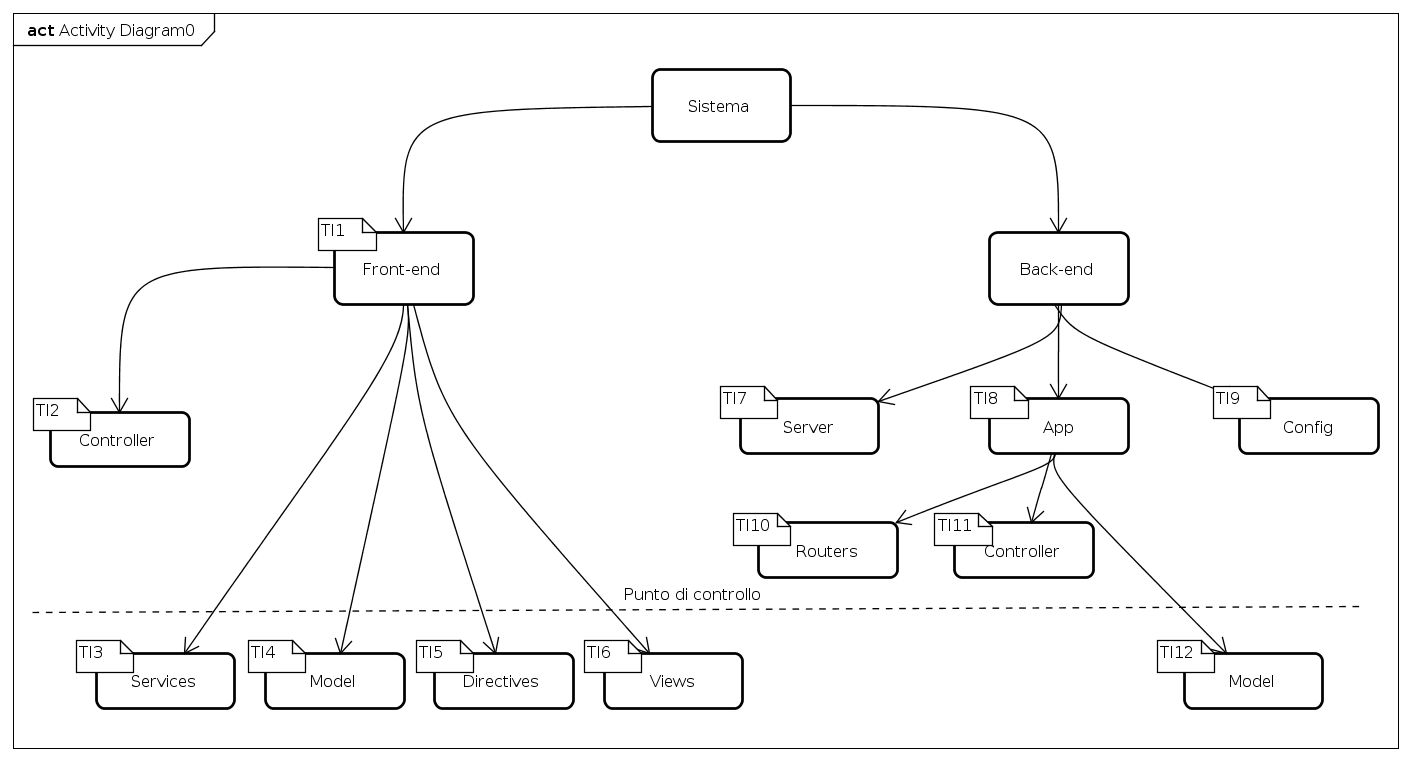
\includegraphics[scale=0.45]{AlberoDiIntegrazione.png}
	\caption{Albero di integrazione delle componenti}
\end{figure}
\FloatBarrier

Nell'approccio top-down dei test di integrazione i moduli di livello più alto vengono sottoposti a test e integrati per primi. Così facendo anche la logica di alto livello e il flusso di dati vengono sottoposti a test fin da subito; sarà perciò necessario simulare le componenti di livello più basso con degli stub. Una volta codificate, le componenti di più basso livello dovranno a loro volta essere integrate e testate. L'approccio top-down rientra tra le strategie di integrazione incrementali, che conferiscono il vantaggio di poter determinare in modo più immediato quale componente causa problemi: i difetti rilevati dai test infatti, nella maggioranza dei casi, saranno da attribuirsi all'ultima componente aggiunta.
\begin{figure}[ht]
	\centering
	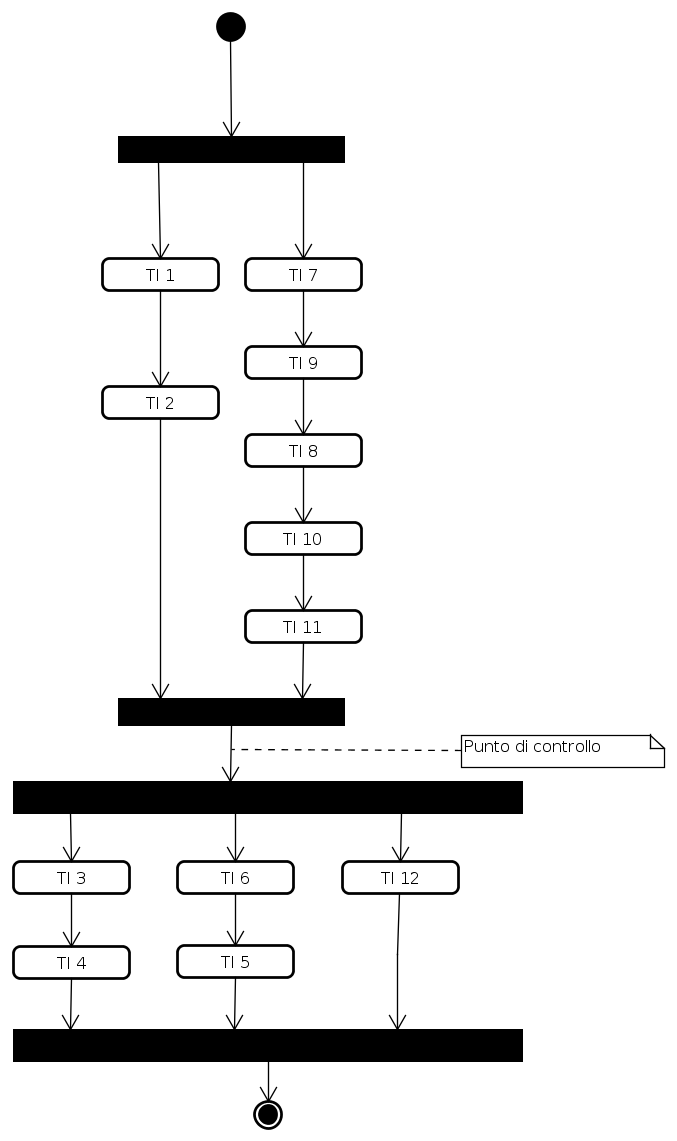
\includegraphics[scale=0.50]{DiagrammaDiAttivita.png}
	\caption{Diagramma di attività dei test di integrazione}
\end{figure}
\FloatBarrier

% TABELLA
\normalsize
\begin{longtable}[ht]{|c|>{}m{10cm}|c|}
\hline 
\textbf{Id Test} & \textbf{Descrizione} & \textbf{Stato}\\
\hline
\endhead
\hypertarget{TI1}{TI1} & Viene verificato che l’applicazione Web gestisca
correttamente il Front-End del prodotto e le sue interazioni
con il Back-End. & \textit{Non Implementato}\\ \hline
\hypertarget{TI2}{TI2} & Viene verificato che i controllers del Front-End si integrino
correttamente nell’applicazione Web. & \textit{Non Implementato}\\ \hline
\hypertarget{TI3}{TI3} & Viene verificato che i services permettano di interagire
correttamente con il Back-End. & \textit{Non Implementato}\\ \hline
\hypertarget{TI4}{TI4} & Viene verificato che il model si integri correttamente con i
services e con le componenti dell’applicazione che lo
utilizzano. & \textit{Non Implementato}\\ \hline
\hypertarget{TI5}{TI5} & Viene verificato che le directives si integrino correttamente
con le views. & \textit{Non Implementato}\\ \hline
\hypertarget{TI6}{TI6} & Viene verificato che le views si integrino correttamente con i
controllers e che visualizzino in modo corretto i dati da essi
ricevuti. & \textit{Non Implementato}\\ \hline
\hypertarget{TI7}{TI7} & Viene verificato che il server si avvii correttamente,
utilizzando \texttt{config} per effettuare le configurazioni
dell’applicazione, e che l’applicazione Web gestisca
correttamente il Back-End del prodotto in modo tale da
fornire al Front-End tutte le informazioni richieste. & \textit{Non Implementato}\\ \hline
\hypertarget{TI8}{TI8} & Viene verificato che \texttt{app} si integri correttamente con le
librerie di Node.js utilizzate. & \textit{Non Implementato}\\ \hline
\hypertarget{TI9}{TI9} & Viene verificato che \texttt{config} si integri con il server, carichi
correttamente tutte le librerie per Node.js che utilizzerà e
che istanzi le classi del package \texttt{app} in modo corretto. & \textit{Non Implementato}\\ \hline
\hypertarget{TI10}{TI10} & Viene verificato che \texttt{config} si integri con il server, carichi
correttamente tutte le librerie per Node.js che utilizzerà e
che istanzi le classi del package \texttt{app} in modo corretto. & \textit{Non Implementato}\\ \hline
\hypertarget{TI11}{TI11} & Viene verificato che i controller si integrino correttamente
e gestiscano le richieste inoltrate dai routers. & \textit{Non Implementato}\\ \hline
\hypertarget{TI12}{TI12} & Viene verificato che il model si integri correttamente con i
controllers per la gestione dell’inserimento, della modifica e
dell’eliminazione dei dati. & \textit{Non Implementato}\\ \hline
\caption[Test di Integrazione]{Test di Integrazione}
\label{tabella:test2}
\end{longtable}
\clearpage
\subsubsection{Test di Unità}
Con questa tipologia di test si vuole verificare il corretto funzionamento delle unità individuate durante la definizione dell'architettura ad alto livello.
I test di unità saranno descritti nel modo seguente:
\begin{center}
\textbf{TU}[\textit{IdTest}]
\end{center}
dove:
\begin{itemize}
\item \textbf{IdTest} rappresenta il codice identificativo crescente dell'unità considerata.
\end{itemize}

% TABELLA
\normalsize
\begin{longtable}{|c|>{}m{10cm}|c|}
\hline 
\textbf{Id Test} & \textbf{Descrizione} & \textbf{Stato}\\
\hline
\endhead
\hypertarget{TU1}{TU1} & Verificare che l’istanza del server venga creata correttamente e che si metta in ascolto su localhost:8080 o che, in caso di errore, la risposta riporti lo stato anomalo riscontrato. & \textcolor{Green}{\textit{Superato}}\\ \hline
\hypertarget{TU2}{TU2} & Verificare che, ricevendo delle richieste conformi alle API definite, l’oggetto passi il controllo al
concreteHandler corretto o che, in caso di errore, la risposta riporti lo stato anomalo riscontrato. & \textit{Non Implementato}\\ \hline
\hypertarget{TU3}{TU3} & Verificare che, in base ai parametri forniti in input, il
JSON ritornato contenga il messaggio d’errore corretto o che, in caso di errore, la risposta riporti lo
stato anomalo riscontrato. & \textit{Non Implementato}\\ \hline
\hypertarget{TU4}{TU4} & Verificare che il messaggio d’errore venga costruito
in modo coerente rispetto ai dati passati al costruttore
e che i metodi disponibili restituiscano l’informazione nel formato desiderato o che, in caso di errore, la
risposta riporti lo stato anomalo riscontrato. & \textit{Non Implementato}\\ \hline
\hypertarget{TU5}{TU5} & Verificare che, in base ai parametri forniti in input, i
metodi effettuino le operazioni richieste, mantenendo
aggiornate le informazioni riguardanti registrazione
ed autenticazione dell’utente o che, in caso di errore,
la risposta riporti lo stato anomalo riscontrato. & \textcolor{Green}{\textit{Superato}}\\ \hline
\hypertarget{TU6}{TU6} & Verificare che, in base ai parametri forniti in input,
il metodo effettui le operazioni richieste, verificando
che l’utente che esegue la richiesta sia effettivamente
un utente autenticato e mantenendo aggiornate le
informazioni riguardanti l’utente
o che, in caso di errore, la risposta riporti lo stato
anomalo riscontrato. & \textcolor{Green}{\textit{Superato}}\\ \hline
\hypertarget{TU7}{TU7} & Verificare che, in base ai parametri forniti in input, i
metodi effettuino le operazioni richieste, mantenendo
aggiornati i dati dell'utente o che, in caso di
errore, la risposta riporti lo stato anomalo riscontrato. & \textcolor{Green}{\textit{Superato}}\\ \hline
\hypertarget{TU8}{TU8} & Verificare che, in base ai parametri forniti in input, i
metodi effettuino le operazioni richieste, mantenendo
aggiornati le statistiche relative all'utente o che, in caso di
errore, la risposta riporti lo stato anomalo riscontrato. & \textcolor{Green}{\textit{Superato}}\\ \hline
\hypertarget{TU9}{TU9} & Verificare che, in base ai parametri forniti in input, i
metodi effettuino le operazioni richieste, mantenendo
aggiornata la cronologia dei questionari svolti o che, in caso di
errore, la risposta riporti lo stato anomalo riscontrato. & \textcolor{Green}{\textit{Superato}}\\ \hline
\hypertarget{TU10}{TU10} & Verificare che, in base ai parametri forniti in input, i metodi effettuino le operazioni richieste, mantenendo aggiornati la gestione dei topic o che, in caso di errore, la risposta riporti lo stato anomalo riscontrato. & \textcolor{Green}{\textit{Superato}}\\ \hline
\hypertarget{TU11}{TU11} & Verificare che, in base ai parametri forniti in input, i metodi effettuino le operazioni richieste, mantenendo aggiornate le statistiche delle domande uscite o che, in caso di errore, la risposta riporti lo stato anomalo riscontrato. & \textcolor{Green}{\textit{Superato}}\\ \hline
\hypertarget{TU12}{TU12} & Verificare che, in base ai parametri forniti in input,
il metodo crei il riepilogo del questionario svolto dall'utente, restituisca il relativo JSON o che, in caso di
errore, la risposta riporti lo stato anomalo riscontrato. & \textcolor{Green}{\textit{Superato}}\\ \hline
\hypertarget{TU13}{TU13} & Verificare che, in base ai parametri forniti in input,
il metodo effettui le operazioni richieste, verificando
che il questionario creato dall'utente sia effettivamente creato 
o che, in caso di errore, la risposta riporti lo stato
anomalo riscontrato. & \textcolor{Green}{\textit{Superato}}\\ \hline
\hypertarget{TU14}{TU14} & Verificare che, in base ai parametri forniti in input, i

metodi effettuino le operazioni richieste, mantenendo

aggiornate le informazioni riguardanti i questionari creati dall'utente
 o che, in caso di errore,
la risposta riporti lo stato anomalo riscontrato. & \textcolor{Green}{\textit{Superato}}\\ \hline
\hypertarget{TU15}{TU15} & Verificare che, in base ai parametri forniti in input, i
metodi effettuino le operazioni richieste, mantenendo
aggiornate le informazioni riguardanti le domande create dall’utente o che, in caso di errore,
la risposta riporti lo stato anomalo riscontrato. & \textcolor{Green}{\textit{Superato}}\\ \hline
\hypertarget{TU16}{TU16} & Verificare che, in base ai parametri forniti in input, i
metodi effettuino le operazioni richieste, verificando che una domanda creata dall’utente sia effettivamente creata o che, in caso di errore, la risposta riporti lo stato anomalo riscontrato. & \textcolor{Green}{\textit{Superato}}\\ \hline
\hypertarget{TU17}{TU17} & Verificare che, in base ai parametri forniti in input, i

metodi effettuino le operazioni richieste, verificando
che le informazioni ottenute per effettuare una traduzione siano corrette o che, in caso di errore,
la risposta riporti lo stato anomalo riscontrato. & \textcolor{Green}{\textit{Superato}}\\ \hline
\hypertarget{TU18}{TU18} & Verificare che, in base ai parametri forniti in input, i
metodi effettuino le operazioni richieste, mantenendo
aggiornate le informazioni dell'utente in modo corretto,
creando un nuovo utente, aggiornandone il contenuto
e restituendone le informazioni nel relativo JSON
o che, in caso di errore, la risposta riporti lo stato anomalo riscontrato. & \textcolor{Green}{\textit{Superato}}\\ \hline
\hypertarget{TU19}{TU19} & Verificare che, in base ai parametri forniti in input, i
metodi effettuino le operazioni richieste, verificando la password inserita in fase di autenticazione
e restituendone un  messaggio di conferma
o che, in caso di errore, la risposta riporti lo stato
anomalo riscontrato. & \textcolor{Green}{\textit{Superato}}\\ \hline
\hypertarget{TU20}{TU20} & Verificare che, in base ai parametri forniti in input, i metodi effettuino le operazioni richieste, mantenendo aggiornate le informazioni di una domanda in modo corretto, creando una nuova domanda, aggiornandone il contenuto e restituendone le informazioni nel relativo JSON o che, in caso di errore, la risposta riporti lo stato anomalo riscontrato. & \textcolor{Green}{\textit{Superato}}\\ \hline
\hypertarget{TU21}{TU21} & Verificare che, in base ai parametri forniti in input, i metodi effettuino le operazioni richieste, mantenendo aggiornate le informazioni di un quiz in modo corretto, creando un nuovo quiz, aggiornandone il contenuto e restituendone le informazioni nel relativo JSON o che, in caso di errore, la risposta riporti lo stato anomalo riscontrato. & \textcolor{Green}{\textit{Superato}}\\ \hline
\hypertarget{TU22}{TU22} & Verificare che, in base ai parametri forniti in input, i metodi effettuino le operazioni richieste, mantenendo aggiornate le informazioni dell'argomento in modo corretto, e restituendone le informazioni nel relativo JSON o che, in caso di errore, la risposta riporti lo stato anomalo riscontrato. & \textcolor{Green}{\textit{Superato}}\\ \hline
\hypertarget{TU23}{TU23} & Verificare che, in base ai parametri forniti in input, i metodi effettuino le operazioni richieste, mantenendo aggiornate le informazioni di un questionario svolto in modo corretto, creando il riepilogo di un questionario svolto e restituendone le informazioni nel relativo JSON o che, in caso di errore, la risposta riporti lo stato anomalo riscontrato. & \textcolor{Green}{\textit{Superato}}\\ \hline
\hypertarget{TU24}{TU24} & Verificare che, in base ai parametri forniti in input, i metodi effettuino le operazioni richieste, mantenendo aggiornate le informazioni delle traduzioni in modo corretto, restituendone le informazioni nel relativo JSON o che, in caso di errore, la risposta riporti lo stato anomalo riscontrato. & \textcolor{Green}{\textit{Superato}}\\ \hline
\hypertarget{TU25}{TU25} & Verificare che il metodo effettui le operazioni richieste, costruendo l’oggetto corrispondente e, per mezzo
di \$routeProvider, associando ad ogni route un controller ed una view o che, in caso di errore, la
risposta riporti lo stato anomalo riscontrato. & \textcolor{Green}{\textit{Superato}}\\ \hline
\hypertarget{TU26}{TU26} & Verificare che il metodo effettui le operazioni richieste, costruendo l’oggetto corrispondente, il quale funge da gestore per gli eventi globali o che, in caso di
errore, la risposta riporti lo stato anomalo riscontrato. & \textcolor{Green}{\textit{Superato}}\\ \hline
\hypertarget{TU27}{TU27} & Verificare che, in base ai parametri forniti in input, i metodi effettuino le operazioni richieste, gestendo i dettagli di un questionario richiamando i metodi del relativo Service. Nello specifico restituendo i dettagli dei questionari creati da un utente e i questionari a cui un utente è iscritto o che, nel caso di errore, la risposta riporti lo stato anomalo riscontrato. & \textcolor{Green}{\textit{Superato}}\\ \hline
\hypertarget{TU28}{TU28} & Verificare che, in base ai parametri forniti in input, i metodi effettuino le operazioni richieste, gestendo tutti i questionari creati da un utente richiamando i metodi del relativo Service. Nello specifico restituendo tutti i questionari creati da un utente o che, nel caso di un errore, la risposta riporti lo stato anomalo riscontrato.  & \textcolor{Green}{\textit{Superato}}\\ \hline
\hypertarget{TU29}{TU29} & Verificare che, in base ai parametri forniti in input, i metodi effettuino le operazioni richieste, gestendo le risposte inserite dall'utente, salvando la domanda inserita dall'utente per poi visualizzarla nella pagina o che, nel caso di un errore, la risposta riporti lo stato anomalo riscontrato. & \textcolor{Green}{\textit{Superato}}\\ \hline
\hypertarget{TU30}{TU30} & Verificare che, in base ai parametri forniti in input, i metodi effettuino le operazioni richieste, gestendo l'autenticazione al sistema, in particolare la richiesta di autenticazione, la richiesta di registrazione e la possibilità di recuperare la password dimenticata o che, nel caso di un errore, la risposta riporti lo stato anomalo riscontrato. & \textcolor{Green}{\textit{Superato}}\\ \hline
\hypertarget{TU31}{TU31} & Verificare che, in base ai parametri forniti in input, i metodi effettuino le operazioni richieste, permettendo di gestire la creazione e la modifica di una domanda ad area cliccabile; in specifico venga controllata la costruzione della relativa domanda e gli eventi che generano la creazione/modifica della domanda  o che, in caso di errore, la risposta riporti lo stato anomalo riscontrato. & \textit{Non Implementato}\\ \hline
\hypertarget{TU32}{TU32} & Verificare che, in base ai parametri forniti in input, i metodi effettuino le operazioni richieste, permettendo di gestire la creazione e la modifica di una domanda a collegamento; in specifico venga controllata la costruzione della relativa domanda e gli eventi che generano la creazione/modifica della domanda o che, in caso di errore, la risposta riporti lo stato anomalo riscontrato. & \textcolor{Green}{\textit{Superato}}\\ \hline
\hypertarget{TU33}{TU33} & Verificare che, in base ai parametri forniti in input, i metodi effettuino le operazioni richieste, gestendo il menù fisso per ogni pagina; in particolare deve gestire il logout dal sistema, il login dal sistema, la registrazione al sistema, la possibilità di effettuare il redirect alla pagina di visualizzazione utente, di gestione profilo utente, di gestione delle domande, di gestione dei questionari e infine gestire la visualizzazione dei giusti collegamenti della barra per ogni pagina o che, nel caso di un errore, la risposta riporti lo stato anomalo riscontrato. & \textcolor{Green}{\textit{Superato}}\\ \hline
\hypertarget{TU34}{TU34} & Verificare che, in base ai parametri forniti in input, i metodi effettuino le operazioni richieste, gestendo la creazione e modifica di domande a risposta multipla, in particolare deve gestire la chiamata al service per l'invio della nuova domanda o che, nel caso di un errore, la risposta riporti lo stato anomalo riscontrato. & \textcolor{Green}{\textit{Superato}}\\ \hline
\hypertarget{TU35}{TU35} & Verificare che, in base ai parametri forniti in input, i metodi effettuino le operazioni richieste, gestendo il redirect alla pagina di creazione di una nuova domanda o che, nel caso di un errore, la risposta riporti lo stato anomalo riscontrato. & \textcolor{Green}{\textit{Superato}}\\ \hline
\hypertarget{TU36}{TU36} & Verificare che, in base ai parametri forniti in input, i metodi effettuino le operazioni richieste, permettendo di gestire la creazione di un nuovo questionario e la modifica di uno esistente; in specifico venga controllata la costruzione del questionario, le operazioni che permettano la conferma creazione/modifica/eliminazione del questionario o che, in caso di errore, la risposta riporti lo stato anomalo riscontrato. & \textcolor{Green}{\textit{Superato}}\\ \hline
\hypertarget{TU37}{TU37} & Verificare che, in base ai parametri forniti in input, i metodi effettuino le operazioni richieste, gestendo il recupero della password dimenticata, in particolare la comunicazione col service per l'invio della mail e la gestione dell'evento redirect alla pagina di login o che, nel caso di un errore, la risposta riporti lo stato anomalo riscontrato. & \textit{Non Implementato}\\ \hline
\hypertarget{TU38}{TU38} & Verificare che, in base ai parametri forniti in input, i metodi effettuino le operazioni richieste, gestendo il recupero delle domande per far si che possano essere visualizzate nella modalità allenamento e nella compilazione di questionari, richiamando i metodi del relativo service. Nello specifico gestendo tutti gli eventi che hanno a che fare con la selezione e la visualizzazione di una nuova domanda o che, nel caso di un errore, la risposta riporti lo stato anomalo riscontrato. & \textcolor{Green}{\textit{Superato}}\\ \hline
\hypertarget{TU39}{TU39} & Verificare che, in base ai parametri forniti in input, i metodi effettuino le operazioni richieste, gestendo il profilo personale dell'utente, in particolare l'invio delle nuove informazioni al service tramite l'apposito metodo. & \textcolor{Green}{\textit{Superato}}\\ \hline
\hypertarget{TU40}{TU40} & Verificare che, in base ai parametri forniti in input, i metodi effettuino le operazioni richieste, gestendo la registrazione di un utente al sistema; in particolare deve richiamare il metodo signup del service AuthService passandogli un oggetto
di tipo SignUpModelView; nel caso di buona riuscita deve essere mostrato un messaggio di successo e gestito il redirect alla pagina di login mentre nel caso contrario deve essere mostrato un messaggio di errore. & \textcolor{Green}{\textit{Superato}}\\ \hline
\hypertarget{TU41}{TU41} & Verificare che, in base ai parametri forniti in input, i metodi effettuino le operazioni richieste, permettendo di gestire la creazione e la modifica di domande create tramite editor QML; in specifico venga controllata la costruzione della domanda e le operazioni che permettano la conferma creazione/modifica della domanda o che, in caso di errore, la risposta riporti lo stato anomalo riscontrato. & \textcolor{Green}{\textit{Superato}}\\ \hline
\hypertarget{TU42}{TU42} & Verificare che, in base ai parametri forniti in input, i metodi effettuino le operazioni richieste, gestendo tutte le domande create da un utente e creandone di nuove richiamando i metodi del relativo service. Nello specifico recuperando tutte le domande create da un utente e gestendo l'evento click sul pulsante di modifica di una domanda o che, nel caso di un errore, la risposta riporti lo stato anomalo riscontrato. & \textcolor{Green}{\textit{Superato}}\\ \hline
\hypertarget{TU43}{TU43} & Verificare che, in base ai parametri forniti in input, i metodi effettuino le operazioni richieste, permettendo di gestire la compilazione del questionario; in specifico venga controllata la visualizzazione del questionario e le operazioni che permettano di rispondere alle varie domanda o che, in caso di errore, la risposta riporti lo stato anomalo riscontrato. & \textcolor{Green}{\textit{Superato}}\\ \hline
\hypertarget{TU44}{TU44} & Verificare che, in base ai parametri forniti in input, i metodi effettuino le operazioni richieste, reagendo ai comandi dell'utente durante la gestione dei suoi questionari richiamando i metodi del relativo service. Nello specifico gestendo l'evento click di modifica/eliminazione/gestione iscrizioni/attivazione modalità esame/allenamento di un questionario o che, nel caso di un errore, la risposta riporti lo stato anomalo riscontrato. & \textcolor{Green}{\textit{Superato}}\\ \hline
\hypertarget{TU45}{TU45} & Verificare che, in base ai parametri forniti in input, i metodi effettuino le operazioni richieste, gestendo le iscrizioni degli utenti ai questionari richiamando i metodi del relativo service. Nello specifico permettendo di iscriversi ad un questionario o che, nel caso di un errore, la risposta riporti lo stato anomalo riscontrato. & \textcolor{Green}{\textit{Superato}}\\ \hline
\hypertarget{TU46}{TU46} & Verificare che, in base ai parametri forniti in input, i metodi effettuino le operazioni richieste, gestendo la visualizzazione dei risultati di un singolo questionario richiamando i metodi del relativo service. Nello specifico restituendo il risultato di un questionario, restituendo tutti gli utenti che hanno eseguito un questionario ed il loro risultato o che, nel caso di un errore, la risposta riporti lo stato anomalo riscontrato. & \textcolor{Green}{\textit{Superato}}\\ \hline
\hypertarget{TU47}{TU47} & Verificare che, in base ai parametri forniti in input, i metodi effettuino le operazioni richieste, gestendo le statistiche di un utente; in particolare deve ottenere tali statistiche attraverso il StatisticsService, passandogli l'username dell'utente ricercato o che, nel caso di un errore, la risposta riporti lo stato anomalo riscontrato. & \textcolor{Green}{\textit{Superato}}\\ \hline
\hypertarget{TU48}{TU48} & Verificare che, in base ai parametri forniti in input, i metodi effettuino le operazioni richieste, permettendo di gestire la creazione e la modifica di una domanda a riempimento di spazi; in specifico venga controllata la costruzione della domanda e le operazioni che permettano la creazione/modifica della domanda o che, in caso di errore, la risposta riporti lo stato anomalo riscontrato. & \textcolor{Green}{\textit{Superato}}\\ \hline
\hypertarget{TU49}{TU49} & Verificare che, in base ai parametri forniti in input, i metodi effettuino le operazioni richieste, permettendo la visualizzazione della homepage; in specifico venga controllata che siano presenti all'interno della home tutte le features previste o che, in caso di errore, la risposta riporti lo stato anomalo riscontrato. & \textcolor{Green}{\textit{Superato}}\\ \hline
\hypertarget{TU50}{TU50} & Verificare che, in base ai parametri forniti in input, i metodi effettuino le operazioni richieste, permettendo di gestire la creazione e la modifica di una domanda a ordinamento immagini; in specifico venga controllata la costruzione della domanda e le operazioni che permettano la creazione/modifica della domanda o che, in caso di errore, la risposta riporti lo stato anomalo riscontrato. & \textcolor{Green}{\textit{Superato}}\\ \hline
\hypertarget{TU51}{TU51} & Verificare che, in base ai parametri forniti in input, i metodi effettuino le operazioni richieste, permettendo di gestire la creazione e la modifica di una domanda a ordinamento di stringhe; in particolare deve gestire l'evento click sul pulsante di conferma sulla domanda, raccogliendo i dati di questa dal modelview e mandandoli al server attraverso il QuestionService; dovrà gestire infine il giusto redirect alla pagina di gestione delle domande oppure al questionario che si stava creando o che, nel caso di un errore, la risposta riporti lo stato anomalo riscontrato. & \textcolor{Green}{\textit{Superato}}\\ \hline
\hypertarget{TU52}{TU52} & Verificare che, in base ai parametri forniti in input, i metodi effettuino le operazioni richieste, gestendo la ricerca di questionari e utenti all'interno dell'applicazione richiamando i metodi del relativo service. Nello specifico gestendo l'evento click sui bottoni per visualizzare l'utente selezionato, per registrarsi ad un questionario, per effettuare una ricerca  o che, nel caso di un errore, la risposta riporti lo stato anomalo riscontrato. & \textcolor{Green}{\textit{Superato}}\\ \hline
\hypertarget{TU53}{TU53} & Verificare che, in base ai parametri forniti in input, i metodi effettuino le operazioni richieste, gestendo il recupero delle parole chiave di un questionario; in particolare data una stringa di ricerca deve restituire la parole chiave associata ad essa o che, nel caso di un errore, la risposta riporti lo stato anomalo riscontrato. & \textcolor{Green}{\textit{Superato}}\\ \hline
\hypertarget{TU54}{TU54} & Verificare che, in base ai parametri forniti in input, i metodi effettuino le operazioni richieste,  gestendo la modalità allenamento sottoponendo all'utente le giuste domande adatte al suo livello; in particolare deve gestire l'evento per inserire una domanda nella cronologia delle domande, gestire l'evento per scaricare una nuova domanda in base ai parametri
passati facendo una richiesta al QuestionsController che andrà a scaricare la domanda e ad inserirla in TrainingModeModel nello \$scope mediante il metodo addQuestion, gestire l'evento per inserire il risultato di una domanda e gestire l'evento per iniziare l'allenamento o, nel caso di un errore, deve garantire che la risposta riporti lo stato anomalo riscontrato. & \textcolor{Green}{\textit{Superato}}\\ \hline
\hypertarget{TU55}{TU55} & Verificare che, in base ai parametri forniti in input, i metodi effettuino le operazioni richieste, permettendo di gestire la creazione e la modifica di una domanda vero e falso; in specifico venga controllata la costruzione della domanda e le operazioni che permettano la creazione/modifica della domanda o che, in caso di errore, la risposta riporti lo stato anomalo riscontrato. & \textcolor{Green}{\textit{Superato}}\\ \hline
\hypertarget{TU56}{TU56} & Verificare che, in base ai parametri forniti in input, i metodi effettuino le operazioni richieste, gestendo i dati di un utente da mostrare nella pagina di un profilo; in particolare deve i dati con una chiamata a UserDetailsService, passandogli l'username dell'utente ricercato o che, nel caso di un errore, la risposta riporti lo stato anomalo riscontrato. & \textcolor{Green}{\textit{Superato}}\\ \hline
\hypertarget{TU57}{TU57} & Verificare che, in base ai parametri forniti in input, i metodi effettuino le operazioni richieste, gestendo i dati di un questionario; in particolare i metodi devono permettere di settare il titolo del questionario, settare l'autore del questionario, ottenere il titolo del questionario, ottenere l'autore del questionario, ottenere la lista di tutte le domande del questionario, aggiungere una domanda al questionario e infine rimuovere una domanda dal questionario o che, nel caso di un errore, la risposta riporti lo stato anomalo riscontrato. & \textcolor{Green}{\textit{Superato}}\\ \hline
\hypertarget{TU58}{TU58} & Verificare che, in base ai parametri forniti in input, i metodi effettuino le operazioni richieste, memorizzando i dati relativi ad un utente e gestendoli richiamando i relativi Controller. Nello specifico gestendo l'autenticazione dell'utente al sistema, la ricerca di questionari e utenti all'interno dell'applicazione, i dati e le statistiche riguardanti un utente o che, nel caso di un errore, la risposta riporti lo stato anomalo riscontrato. & \textcolor{Green}{\textit{Superato}}\\ \hline
\hypertarget{TU59}{TU59} & Verificare che i metodi getter effettuino le operazioni
richieste, restituendo i dati necessari per la creazione dinamica della barra
menù posizionata in modo fisso su ogni pagina; o che, in caso di errore, la risposta riporti lo
stato anomalo riscontrato. & \textcolor{Green}{\textit{Superato}}\\ \hline
\hypertarget{TU60}{TU60} & Verificare che, in base ai parametri forniti in input,
i metodi effettuino le operazioni richieste, costruendo l’oggetto contenente le informazioni sull'errore,
ritornando correttamente il titolo, il messaggio ed il
codice dell’errore o che, in caso di errore, la risposta
riporti lo stato anomalo riscontrato. & \textcolor{Green}{\textit{Superato}}\\ \hline
\hypertarget{TU61}{TU61} & Verificare che, in base ai parametri forniti in input, i metodi effettuino le operazioni richieste, gestendo i dati di una domanda; in particolare i metodi devono permettere di settare l'autore, settare il metodo con il quale è stata creata, settare la lingua, settare tutte le parti della domanda, settare l'id della domanda con quello ottenuto automaticamente, ottenere l'autore, ottenere il metodo con il quale è stata creata, ottenere la lingua, ottenere l'oggetto domanda, ottenere l'id della domanda, comparare le risposte date con quelle corrette, aggiungere un pezzo nuovo di domanda e creare una domanda o, nel caso di un errore, deve garantire la risposta riporti lo stato anomalo riscontrato. & \textcolor{Green}{\textit{Superato}}\\ \hline
\hypertarget{TU62}{TU62} & Verificare che, in base ai parametri forniti in input, i metodi effettuino le operazioni richieste, memorizzando i dati di un alenamento e gestendoli richiamando il relativo Controller. Nello specifico settando/recuperando argomento, numero di domande dell'allenamento, inserendo/rimuovendo una domanda, aggiungendo/rimuovendo una parola chiave, recuperando il riepilogo dell'allenamento o che, nel caso di un errore, la risposta riporti lo stato anomalo riscontrato. & \textcolor{Green}{\textit{Superato}}\\ \hline
\hypertarget{TU63}{TU63} & Verificare che, in base ai parametri forniti in input,
i metodi effettuino le operazioni richieste, costruendo l’oggetto contenente riguardanti la giusta traduzione dell’applicazione, ritornando correttamente la lingua, la lista di keywords o che, in caso di errore, la risposta riporti lo stato anomalo riscontrato. & \textcolor{Green}{\textit{Superato}}\\ \hline
\hypertarget{TU64}{TU64} & Verificare che, in base ai parametri forniti in input,
i metodi effettuino le operazioni richieste, costruendo l’oggetto contenente riguardanti la giusta traduzione dell’applicazione, impostando correttamente la nuova lingua inserita o che, in caso di errore, la risposta riporti lo stato anomalo riscontrato. & \textcolor{Green}{\textit{Superato}}\\ \hline
\hypertarget{TU65}{TU65} & Verificare che, in base ai parametri forniti in input, i metodi effettuino le operazioni richieste, gestendo le domande, ossia il loro recupero e salvataggio; in particolare i metodi devono permettere di inviare una richiesta di salvataggio di una domanda, ottenere tutte le domande di un utente, ottenere le keywords a partire da una stringa in input, ritornare una singola domanda avendo come input l'id e infine ottenere la domanda successiva per la modalità allenamento o, nel caso di un errore, deve garantire che la risposta riporti lo stato anomalo riscontrato. & \textcolor{Green}{\textit{Superato}}\\ \hline
\hypertarget{TU66}{TU66} & Verificare che, in base ai parametri forniti in input, i metodi effettuino le operazioni richieste, gestendo la registrazione e l'autenticazione di un utente fornendone le funzionalità ai Controller. Nello specifico permettendo di controllare se un utente è già autenticato, di effettuare il login, il logout, la registrazione e il recupero della password o che, nel caso di un errore, la risposta riporti lo stato anomalo riscontrato. & \textcolor{Green}{\textit{Superato}}\\ \hline
\hypertarget{TU67}{TU67} & Verificare che, in base ai parametri forniti in input, i metodi effettuino le operazioni richieste, gestendo la lingua in cui un utente ha deciso di utilizzare un'applicazione e fornendo le funzionalità per recuperare la giusta traduzione delle pagine. Nello specifico recuperando la lista di tutte le keywords nella lingua richiesta o che, nel caso di un errore, la risposta riporti lo stato anomalo riscontrato. & \textcolor{Green}{\textit{Superato}}\\ \hline
\hypertarget{TU68}{TU68} & Verificare che, in base ai parametri forniti in input, utilizzando il service SearchService, i metodi richiedano in maniera corretta le informazioni inerenti alla ricerca degli utenti e dei questionari, che i dati vengano restituiti nella maniera attesa o che, in caso di errore, la risposta riporti lo stato anomalo riscontrato. & \textcolor{Green}{\textit{Superato}}\\ \hline
\hypertarget{TU69}{TU69} & Verificare che, in base ai parametri forniti in input, i metodi effettuino le operazioni richieste, gestendo tutto ciò che riguarda i questionari; in particolare i metodi devono permettere di cercare un questionario, iscrivere un utente ad un questionario, ottenere tutti i dettagli di un questionario, ottenere tutti i questionari eseguiti da un utente, creare un nuovo questionario, ottenere tutti i questionari creati da un utente, ottenere tutti i questionari a cui un utente è iscritto, approvare l'iscrizione di un utente ad un questionario, ottenere tutti gli utenti che hanno eseguito un particolare questionario, ottenere i risultati di un questionario e infine ottenere i risultati di un singolo utente ad un questionario o, nel caso di un errore, deve garantire che la risposta riporti lo stato anomalo riscontrato. & \textcolor{Green}{\textit{Superato}}\\ \hline
\hypertarget{TU70}{TU70} & Verificare che, in base ai parametri forniti in input, utilizzando il service StatisticsService, i metodi richiedano in maniera corretta le informazioni inerenti alle statistiche degli utenti e dei questionari, che i dati vengano restituiti nella maniera attesa o che, in caso di errore, la risposta riporti lo stato anomalo riscontrato. & \textcolor{Green}{\textit{Superato}}\\ \hline
\hypertarget{TU71}{TU71} & Verificare che, in base ai parametri forniti in input, utilizzando il service UserDetailsService, i metodi richiedano in maniera corretta l'ottenimento  e il salvataggio dei dati dell'utente, che i dati vengano restituiti nella maniera attesa o che, in caso di errore, la risposta riporti lo stato
anomalo riscontrato. & \textcolor{Green}{\textit{Superato}}\\ \hline
\caption[Test di Unità]{Test di Unità}
\label{tabella:test3}
\end{longtable}
\clearpage